\documentclass[11pt, a4paper]{article}
\usepackage[utf8x]{inputenc}
\usepackage[swedish, english]{babel}		% last is active
\usepackage{graphicx}
\usepackage{amsmath}					% to be able to \split eqs
\usepackage{amssymb}					% Real/Imaginary fonts
\usepackage{units}
\usepackage[tight, hang]{subfigure}
\usepackage{url}
\usepackage{tikz}						% for drawing
\usetikzlibrary{shapes, arrows, decorations.markings, decorations.pathmorphing, decorations.pathreplacing, calc}
\usepackage{fancyhdr}
\usepackage{float}						% H-positioned and custom floats
\usepackage{datetime}					% to fix date format
\usepackage[usenames,dvipsnames]{pstricks}
%\usepackage{epsfig}
%\usepackage{pst-grad} % For gradients
%\usepackage{pst-plot} % For axes
\usepackage{pgfplots}
% =================== some local stuff ================= %
\newcommand{\degree}{\ensuremath{^\circ}}
\newcommand{\todayswe}{\the\year-\twodigit\month-\twodigit\day}


\def\contacts{Torbjørn Ludvigsen, tolu0022@student.umu.se\\Olof Lenti, olle0004@student.umu.se\\
Yunus Gures, yunusgures@gmail.com}
\def\names{Torbjørn Ludvigsen, Olof Lenti, Yunus Gures}
\def\dept{Department of Physics}
\def\course{Non-invasive measurement techniques}
\def\lab{Optical measurements:\\Determination of the Damping of a Pendulum with Time of Flight}
\def\supervisors{Patrick Ehlers\\Isak Silander\\ Amir Khodabakhsh}
\date{\todayswe}
% custom commands
\newcommand\OpVec[1]{\boldsymbol{\hat{#1}}}		% bold with hat for operator vectors
%\newcommand\Sup[1]{\textsuperscript{\tiny{#1}}}		% 1st, 2nd.. and so on
\newenvironment{eqn}{\begin{equation*} \begin{split}}{\end{equation*} \end{split}}
% header

% document
\begin{document}
\pagestyle{fancy}
\begin{titlepage}
	\begin{center}
		\course\\
		\Large{\lab}\vspace{2mm}
		\hrule\vspace{2mm}
		\tiny{\contacts}\vspace{2mm}
		\hrule
	\end{center}
	\vspace{4mm}

	\begin{abstract}

  $\alpha_{alu} =\unit[(23.0 \pm 0.1)\cdot10^{-6}]{K^{-1}}$ 

  $\alpha_{sst} = \unit[(15.8 \pm 0.2)\cdot10^{-6}]{K^{-1}}$, 
    which is only 1 \% off tabulated values \cite{ph, thex}.

	\end{abstract}
	\vfill
	\hrule\vspace{2mm}
	\centering
		\tiny{Supervisor: \supervisors}
	%\end{center}
\end{titlepage}

\pagestyle{plain}
\vspace{2cm}
\section{Introduction}
A mechanical system cosisting only of a rigid body, with only one degree of 
freedom, rotation around a constant axis, from here on called a pendulum, is 
a system of great interest. Historically it has had a wide range of
applications in science, mathemathics and in everyday life. Among the reasons for
its continued importance as an educational tool in physics is its short, general 
equations of
motion in the linearized, small amplitude case, and the ease and the great number 
of ways by which this case can be extended.

This experiment in particular will measure a physical pendulum's decreasing velocity
in order to find and analyze its damping forces. A time of flight instrumentation
is constructed and used to aquire the velocity data.

\section{Theory}
\subsection{Time of Flight}
Time of Flight (ToF) is a method that measures the time for an object to move a known distance.
You can find the distance of an object or velocity or path length of a movement with this technique.
We convert this technique to find velocity of pendulum. We have two parallel beams 
with optic setup. Pendulum make a harmonic oscillator between these beams. We know the 
distance between two beams. We take time data with photodiodes. When pendulum pass the 
beams, that cause picks at DAQ data. We can get time values with measure distance between 
these picks.
\subsection{The pendulum}
For a simple rigid body pendulum, using Newtons second law and balancing the
forces gives us the following
equation of motion:
\begin{equation}
  \frac{d^2\theta}{dt^2} + \frac{mgl\sin{\theta}}{I_p} = 0,
  \label{eq_of_motion}
\end{equation}
where $I_p$ is the bodys moment of inertia around the pivot point, $\theta$ is the
angle between the line through the pivot and the bodys center of mass and the
vertical line, $m$ is the mass, $g$ is the acceleration due to gravity and
$l$ is the distance from the pivot to the center of mass.


%By approximating $\sin{\theta} \approx \theta$, we
%get the simpler expression
%\begin{equation}
%  \theta = Ae^{r_1t} + Be^{r_2t},
%  \label{diff_solution}
%\end{equation}
%where $A$, $B$ are constant determined by initial conditions and $r_1$, $r_2$ are
%solutions to the second order polynomial created by substituting equation
%\ref{diff_solution} into \ref{eq_of_motion}.

\subsubsection{Introducing Friction}
A physical pendulum will usually experience some friction between solid
surfaces around its pivot point.
This force may sometimes be modelled as being proportional to velocity\cite[p. 30]{book},
and sometimes as independent of velocity \cite{friction}.

To both of these dependencies into \ref{eq_of_motion}, 
we introduce a term $F_l = -a \frac{d\theta}{dt} - c$ into it. 
\begin{equation}
    \frac{d^2\theta}{dt^2} 
  - A \frac{d\theta}{dt}
  + \frac{mgl}{I_p}\sin{\theta} = \text{sgn}(\frac{d\theta}{dt})C,
  \label{eq_of_motion_comp1}
\end{equation}
where $A$ and $C$ are constants.
If $C = 0$ this now discribes the motions of what is 
called a damped harmonic oscillator\cite{osc}.

\subsubsection{Introducing Drag}
Air drag is the force between the air and the pendulum. 
This force is highly dependent on velocity.
For low velocities we approximate the air to be small evenly distributed balls, bouncing off the
pendulum as it travels through space. 
Increasing velocity by some factor will increase the number of bouncing by the same
factor, so this introduces a linear term into 
Equation \ref{eq_of_motion_comp1}, and can be accounted for by adjusting the constant
$A$.

For higher velocities, however, this model breaks down, and the air must be
modelled as a fluid. Drag forces in fluids are proportional to the velocity
squared\cite{drag}, which for us means inserting a force 
$F_D = -B\cdot \left(\frac{d\theta}{dt}\right)^2$, where $B$ is a constant,
into Equation \ref{eq_of_motion_comp1}, giving us the equation of motion

\begin{equation}
    \frac{d^2\theta}{dt^2} 
  - B \frac{d\theta}{dt}
  + \left(1 + \frac{B}{A} \frac{d\theta}{dt} \right)  
  + \frac{mgl}{I_p}\sin{\theta} = \text{sgn}(\frac{d\theta}{dt})C,
  \label{eq_of_motion_comp2}
\end{equation}

It looks like a damped harmonic oscillator, but with a
damping ratio that depends on velocity. 

At the pendulums lowest point we have, $\theta = \sin{\theta} = 0$



\subsection{Optics}
\subsection{Circuits}


\section{Experimental Setup}
The experimental setup consists of one electric circuit described in section \ref{s:Electric circuit}, one optical setup described in \ref{s:Optical setup} and a PC with MATLAB and LabVIEW installed. 
The setup can be seen in Figure \ref{f:setup}. 

\begin{figure}[h]
	\centering
	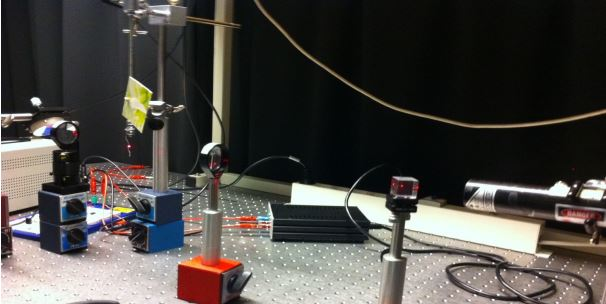
\includegraphics{setup}
	\caption{The electric circuit of the setup. D1 and D2 are the photodiodes.}
	\label{f:setup}
\end{figure}

\subsection{Electric circuit}
\label{s:Electric circuit}
The first mission is to convert light to voltage. This is done by using photodiodes that converts light into current, which is then converted using a current-to-voltage converter.
Photodiodes are made from semiconductor materials and are based on p-n junction principle. We use Silicon photodiodes in the experiment. The electric circuit can be seen in Figure \ref{f:circuit}.
\begin{figure}[h]
	\centering
	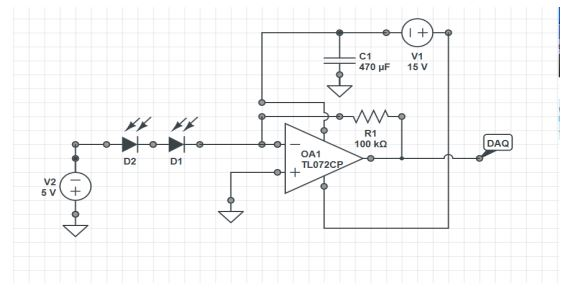
\includegraphics{circuit}
	\caption{The electric circuit of the setup. D1 and D2 are the photodiodes.}
	\label{f:circuit}
\end{figure}

We connect a 100k resistor from input to output to create an inverting amplifier. We feed the operational amplifier with 15V and we use 470µF capacitor to reduce noise. The voltage is digitalized by a DAQ card that we attach to output of the amplifier. LabVIEW is used to collect the data.

\subsection{Optical setup}
\label{s:Optical setup}
The optical setup can be seen in Figure \ref{f:opticalsetup}. We use a Helium-Neon  laser(JDSU 1101) with a wavelength of 632,8nm. Firstly we set the laser, beam splitter, lenses and mirror on the same height. We get two parallel beams with the beam splitter. 
We mount a wire to our pendulum. Because pendulum is too thick to get well data. Then we paint the wire with tipp-ex to prevent beam reflection from it. We use a straight mirror to angle the beam to photodiodes. We put two +100 lens to get more clear beams.

\begin{figure}[h]
	\centering
	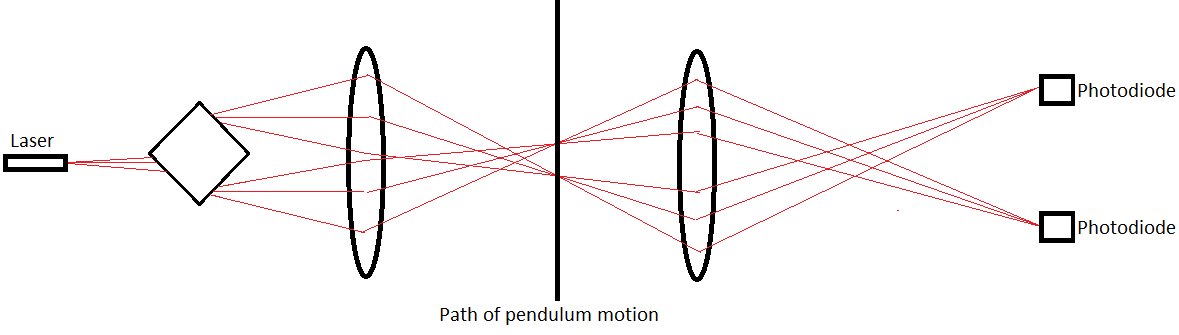
\includegraphics[scale=0.4]{opticalsetup2}
	\caption{The optical setup seen from above. A mirror is also used to direct the lasers onto the photodiodes. The figure is not correct according to scale.}
	\label{f:opticalsetup}
\end{figure}

\section{Procedure}

\section{Error calculations}

\subsection{Error of the slope of a linear fitting}
To calculate the error of the slope of a linear fit we simply use MATLAB to calculate the following equation:
\begin{equation}
	s = \text{std}(f(x)-data(x)),
	\label{e:std}
\end{equation}
where $s$ is the standard deviation of the residuals, $x$ is the x-values of the region considered, 
$data$ is the data values of the region considered and $f$ is the linear fit.
This standard deviation will be a measure of how correct the linear approximation is, 
but also gives an approximation of the total error from the time of flight intrumentation.

\section{Results}
In Figure \ref{f:nopaper} we see the logarithm of work done by the friction and 
drag on the pendulum plotted versus the logarithm of velocity. 
The units of the work and velocity are a constant times their SI-unit. 
The slopes and the errors of the linear fits of the two different regions of the plot are calculated to be
\[
	slope_{low}=\frac{\Delta\ln(W_{low})}{\Delta\ln(v_{low})} = 1.36(4),
\]\[
	slope_{high}=\frac{\Delta\ln(W_{high})}{\Delta\ln(v_{high})} = 2.60(3).
\]
The values inside the parentheses are the standard deviation of the slope calculated using Equation \ref{e:std}.

\begin{figure}[h]
	\centering
	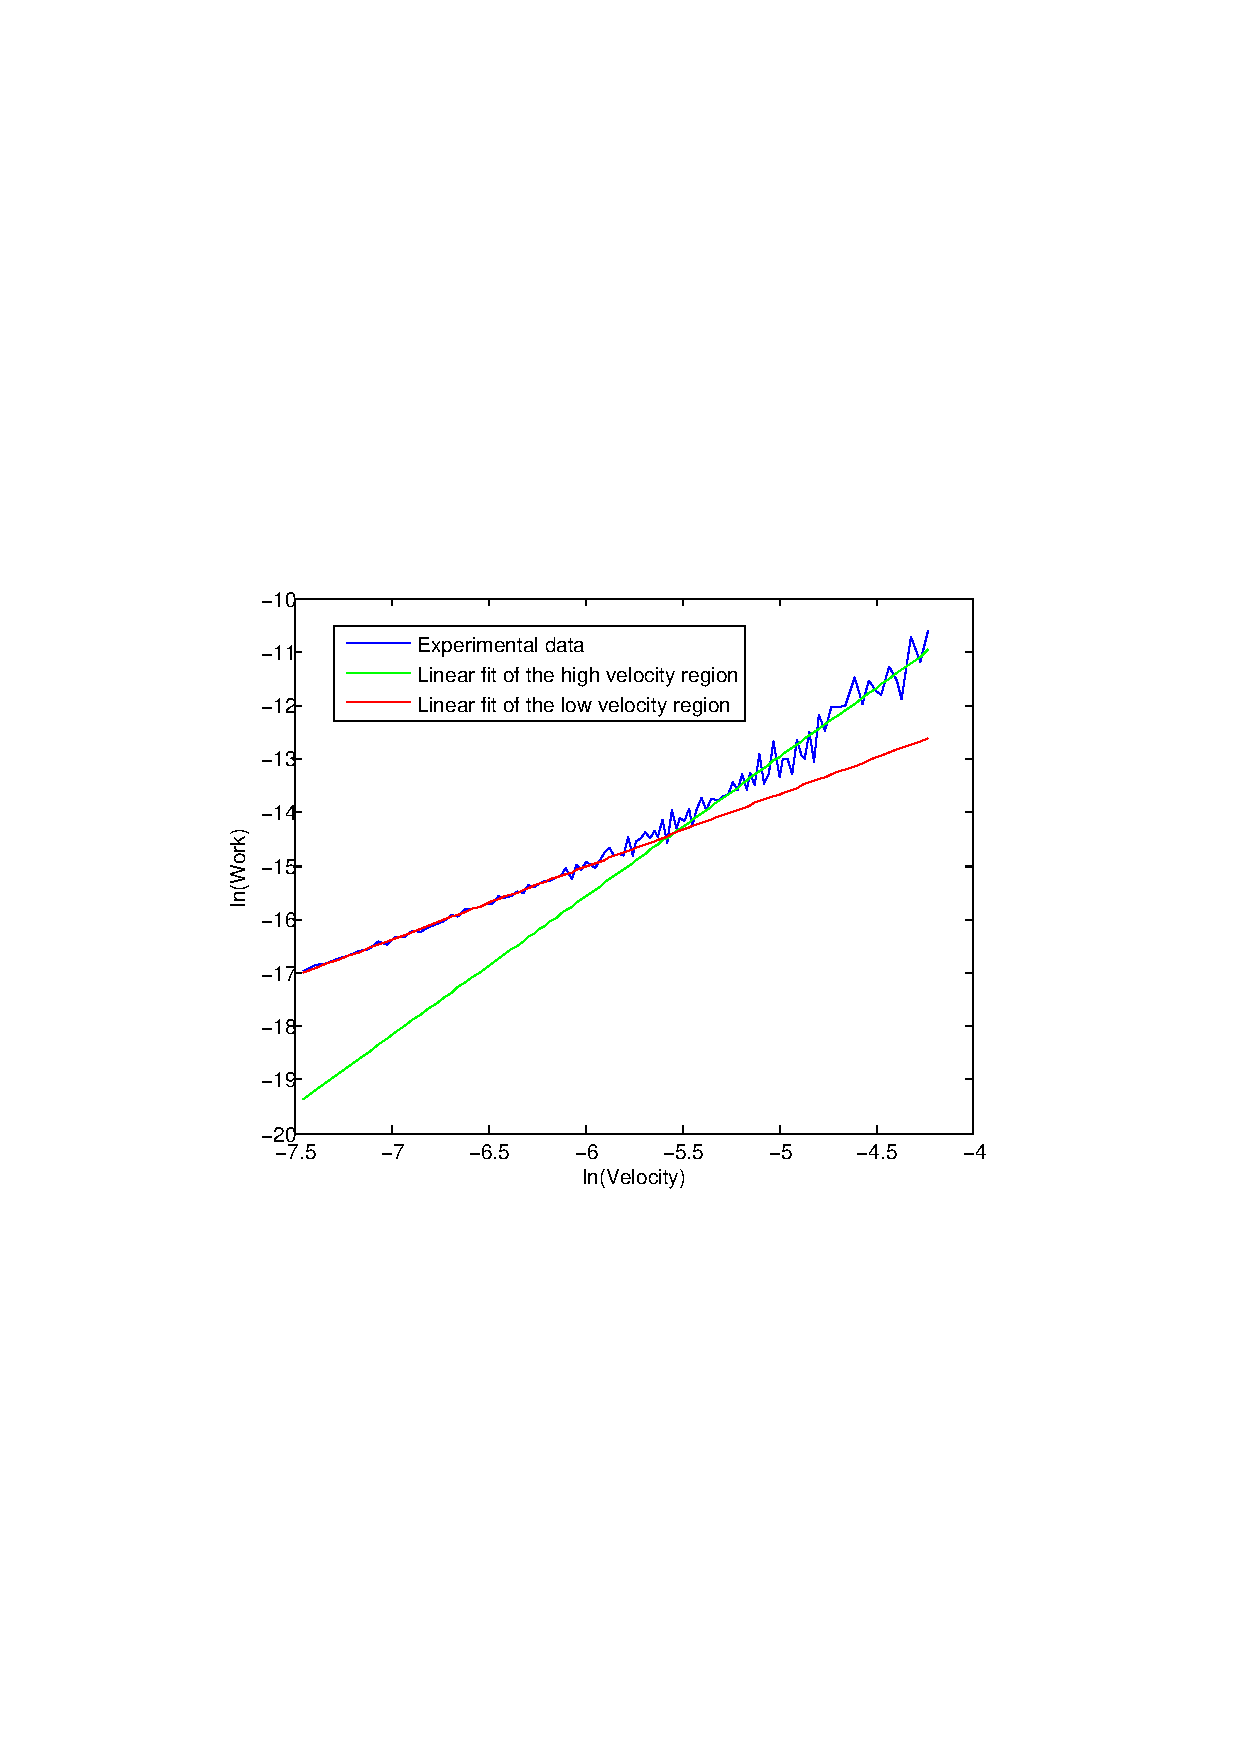
\includegraphics[trim=10.0cm 10.0cm 10.0cm 10.0cm, scale=0.7]{no_paper}
	\caption{Work versus velocity data and  linear fits for the pendulum.}
	\label{f:nopaper}
\end{figure}

In Figure \ref{f:paper} we see the logarithm of work done by the friction and 
drag on the pendulum with the added area plotted versus the logarithm of velocity. 
The units of the work and velocity are a constant times their SI-unit. 
The slopes and the errors of the linear fits of the two different regions of the plot are calculated to be

\[
	slope_{low}=\frac{\Delta\ln(W_{low})}{\Delta\ln(v_{low})} = 1.96(4),
\]\[
	slope_{high}=\frac{\Delta\ln(W_{high})}{\Delta\ln(v_{high})} = 2.63(7).
\]

\begin{figure}[h]
	\centering
	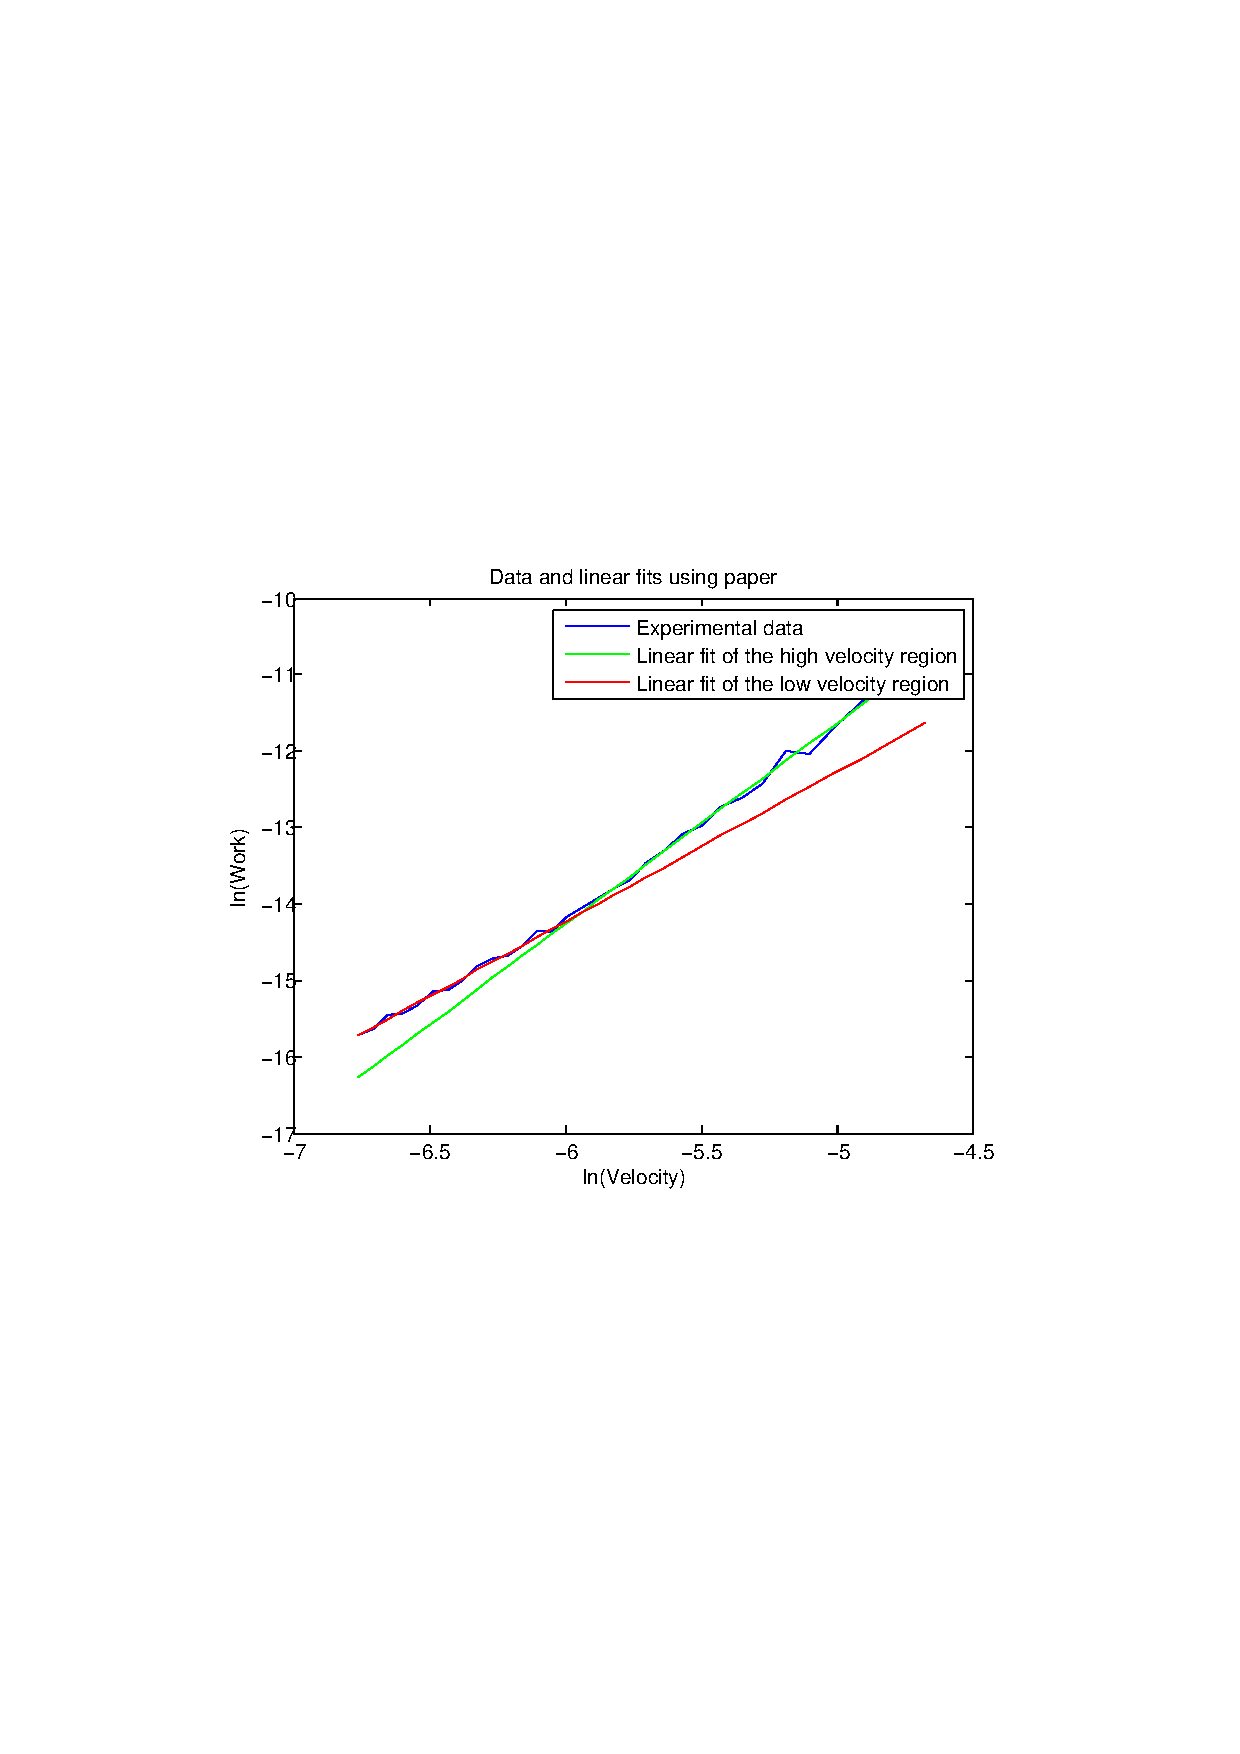
\includegraphics[trim=10.0cm 10.0cm 10.0cm 10.0cm, scale=0.7]{paper}
	\caption{Work versus velocity data and  linear fits for the pendulum with an added area.}
	\label{f:paper}
\end{figure}

It is clear that the slopes of the high velocity region are similar and close to $3$. 
The slope of the added-area pendulum for the low-velocity region is very close to $2$.
The slope of the ordinary pendulum for the low-velocity region is slightly above $1$.



\section{Discussion}
The experimentally retrieved plots values are very precise and describing. They demonstrate the three types of frictional forces of 

The behavior of the high-velocity region is not entirely as expected. We expected the slope of the added-area pendulum 
to be closer to $3$ than the other pendulum.
This is explained by the fact that the high-velocity regions are not exactly the same for the different types of pendula. We were not 
able to do a high enough velocity measurement due to the quick damping as well as the fluttering of the added area.
\section{Summary and Conclusions}
\vfill

\begin{thebibliography}{99}
	\bibitem{ph} Nordling, C., Österman, J. (2006). 
  \textit{Physics Handbook  $8^{th}$}\\
  Lund, Sweden, Studentlitteratur.

  \bibitem{drag} Wikipedia. \textit{Drag}\\ 
  \url{http://en.wikipedia.org/wiki/Drag_(physics)} [\todayswe]

  \bibitem{osc} Wikipedia. \textit{Harmonic oscillator}\\ 
  \url{http://en.wikipedia.org/wiki/Harmonic_oscillator} [\todayswe]

	\bibitem{book} Baker, Blackburn (2005). 
  \textit{The Pendulum, A Case Study in Physics}\\
  Oxford, University Press.

  \bibitem{friction} Wikipedia. \textit{Friction}\\ 
  \url{http://en.wikipedia.org/wiki/Friction} [\todayswe]

\end{thebibliography}

\begin{appendix}
\end{appendix}

% nY KOMMENTAR

\end{document}
%\begin{figure}[H]
%	\centering
%	\begin{tikzpicture}[scale = 0.95]
%		\def\mr{1.5};
%		\draw (0,0) ellipse (0.5 and \mr);
%		\begin{scope}
%			\clip (0,0) ellipse (0.5 and \mr);
%			\foreach \i in {0, 1, ..., 15} {
%				\draw (-0.5, {-3 + 0.25*\i}) -- (0.5, {-1 + 0.25 * \i});
%			}
%		\end{scope}
%		\path[fill = white, opacity = 0.7] (0, 0) circle (0.2);
%		\node at (0, 0) {$S$};
%		\begin{scope}
%			% overlapping regions will cancel out
%			\draw[fill = white] (5, 0) circle (3);
%		\end{scope}
%		\draw (0, \mr) -- ++(2.8, 0) to[out = 0, in = -135] ++(0.3, 0.3)
%			  (0, -\mr) -- ++(2.8, 0) to[out = 0, in = 135] ++(0.3, -0.3);
%		\node at (5, 0) {$V$};
%	\end{tikzpicture}
%	\caption{Helmholtz resonator}
%	\label{f:helmholtz}
%\end{figure}
